\documentclass[a4paper,10pt]{article}
\usepackage{%
	amsfonts,%
	amsmath,%	
	etex,%
	amssymb,%
	amsthm,%
	babel,%
	bbm,%
	%biblatex,%
	caption,%
	centernot,%
	color,%
	enumerate,%
	epsfig,%
	epstopdf,%
	geometry,%
	graphicx,%
	hyperref,%
	latexsym,%
	mathtools,%
	multicol,%
	pgf,%
	pgfplots,%
	pgfplotstable,%
	pgfpages,%
	proof,%
	psfrag,%
	subfigure,%	
	tikz,%
	ulem,%
	url%
}	

\usepackage[mathscr]{eucal}
\usepgflibrary{shapes}
\usetikzlibrary{%
  arrows,%
	backgrounds,%
	chains,%
	decorations.pathmorphing,% /pgf/decoration/random steps | erste Graphik
	decorations.text,%
	matrix,%
  	positioning,% wg. " of "
  	fit,%
	patterns,%
  	petri,%
	plotmarks,%
  	scopes,%
	shadows,%
  	shapes.misc,% wg. rounded rectangle
  	shapes.arrows,%
	shapes.callouts,%
  	shapes%
}

\theoremstyle{plain}
\newtheorem{thm}{Theorem}[section]
\newtheorem{lem}[thm]{Lemma}
\newtheorem{prop}[thm]{Proposition}
\newtheorem{cor}[thm]{Corollary}

\theoremstyle{definition}
\newtheorem{defn}[thm]{Definition}
\newtheorem{conj}[thm]{Conjecture}
\newtheorem{exmp}[thm]{Example}
\newtheorem{assum}[thm]{Assumptions}
\newtheorem{axiom}[thm]{Axiom}

\theoremstyle{remark}
\newtheorem{rem}{Remark}
\newtheorem{note}{Note}

\newcommand{\norm}[1]{\left\lVert#1\right\rVert}
\newcommand{\indep}{\!\perp\!\!\!\perp}
\DeclarePairedDelimiter\abs{\lvert}{\rvert}%
%\DeclarePairedDelimiter\norm{\lVert}{\rVert}%
\newcommand{\tr}{\operatorname{tr}}
\newcommand{\R}{\mathbb{R}}
\newcommand{\Q}{\mathbb{Q}}
\newcommand{\N}{\mathbb{N}}
\newcommand{\E}{\mathbb{E}}
\newcommand{\Z}{\mathbb{Z}}
\newcommand{\B}{\mathscr{B}}
\newcommand{\C}{\mathcal{C}}
\newcommand{\T}{\mathscr{T}}
\newcommand{\F}{\mathcal{F}}
\newcommand{\G}{\mathcal{G}}
%\newcommand{\ba}{\begin{align*}}
%\newcommand{\ea}{\end{align*}}

\makeatletter
\def\th@plain{%
  \thm@notefont{}% same as heading font
  \itshape % body font
}
\def\th@definition{%
  \thm@notefont{}% same as heading font
  \normalfont % body font
}
\makeatother
\date{}
\title{Lecture 3:  Compound Poisson Process}
\author{Parimal Parag}

\begin{document}
\maketitle

\section{Compound Poisson Process}
One of the characterizations of Poisson process was single arrival in an infinitesimal time. We can generalize that definition to have a random number of arrivals $X_n$ at every arrival instant $S_n$.
\begin{defn}[Compound Poisson process] Let $\left\{X_i\right\}$ be \emph{iid} random variables. Let $N(t), t\geq 0$ be a Poisson Process with parameter $\lambda$ independent of $X_i, i\geq 1$. Then the process $X(t)$ defined as
\begin{equation*}
X(t) = \sum_{i=1}^{N(t)} X_i
\end{equation*}
is called a \textbf{compound Poisson process}.
\end{defn}
We derive some properties of compound Poisson Processes in the following.
\subsection{Mean}
\begin{align*}
E[X(t)] = E[\sum_{i=1}^{N(t)} X_i] &= E[E[\sum_{i=1}^{N(t)} X_i|N(t)]] \\
&= \sum_{k=0}^\infty E\left[\sum_{i=1}^{k} X_i|N(t)=k\right]\Pr\{N(t) = k\}\\
&= \sum_{k=0}^\infty \sum_{i=1}^{k} E[X_i]\Pr\{N(t) = k\}\\
&= E[N(t)]E[X_1] = \lambda tE[X_1].
\end{align*}

\subsection{MGF}
We leave it as an exercise to show that $M_{X(t)}(\theta)=E[e^{\theta X(t)}] = e^{(M_X(\theta)-1)\lambda t}$.

\subsection{A nice counterexample}
A Poisson process is not uniquely determined by it's distribution. Let $X_t = Y_t + f(Z+t)$, where $Y_t$ is a Poisson Process and 
\begin{equation*}
f(t) = t 1_{\{t \in \mathbb{Q}\}}.
\end{equation*}
Let $Z$ be a continuous random variable. Then we can show that $\Pr\{X_t \neq Y_t) = 0$. This is true since
\begin{flalign*}
\Pr\{X_t \neq Y_t\} &= \Pr\{\omega \in \Omega: \quad t+Z(\omega) \in \mathbb{Q}\} \\
&= \Pr\{\omega \in \Omega:  Z(\omega) \in \mathbb{Q} - t\} = 0.
\end{flalign*}
The last part follows since $\mathbb{Q}-t$ is a countable set of individual events with probability zero. We can also show that $X(t)$ and $Y(t)$ have same fdds.
\begin{equation*}
  \Pr\{X_{t_1}= Y_{t_1}, X_{t_2}= Y_{t_2}\}
  = \sum_{n_{1},n_{2}}\Pr\{X_{t_1} = n_1, X_{t_2}= n_2, Y_{t_1}=n_1, Y_{t_2}=n_2 \}  = 1.
\end{equation*}
$\{X_{t}(\omega)\}$ can take non-integer values and is not non-decreasing. Two process can have same distribution but sample path behavior can be quite different.
%\section{Compound (Batch) Poisson Process}
%
%\begin{eqnarray*}
%% \nonumber to remove numbering (before each equation)
  %N_{t} &=& \sup \{n: S_{n}\leq t \}  \\
  %\end{eqnarray*}
   %$\overline{N_{t}}$= No of arrivals till time $n$  \\
   %\begin{eqnarray*}
   %\overline{N_{t}}&=& \sum ^{N_{t}}_{k=0}Z_{k}  ~(\text{No. of arrivals till time $n$}).\\
   %\mathbb{E}[\overline{N_{t}}]&=&\mathbb{E}\left[\sum ^{N_{t}}_{k=0}Z_{k}\right]  \\
   %&=& \sum^{\infty}_{n=0}\mathbb{E}\left[\sum ^{N_{t}}_{k=0}Z_{k}|N_{t}-n \right] P[N_{t}=n]\\
   %&=& \sum^{\infty}_{n=0}P[N_{t}=n]\mathbb{E}\left[\sum^{\infty}_{k=0}Z_{k}|N_{t}=n   \right] \\
   %&=& \sum^{\infty}_{n=0} \frac{e^{-\lambda t} (\lambda t)^{n}}{n!} n \mathbb{E}[Z_{1}] \\
   %&=& \mathbb{E} [Z_{1}]\mathbb{E} [N_{t}].
   %\end{eqnarray*}
   %For  $  \alpha>0 $,  \\
   %\begin{eqnarray*}
   %&\mathbb{E}[e^{\alpha \overline{N_{t}}}]=\mathbb{E}\left[e^{\alpha\sum ^{N_{t}}_{k=0}Z_{k}}\right] \\
   %&=& \sum^{\infty}_{n=0}\mathbb{E}\left[ e^{\alpha\sum ^{N_{t}}_{k=0}Z_{k}}| N_{t}=n\right] P[N_{t}=n]\\
   %&=&  \sum^{\infty}_{n=0}\mathbb{E}\left[e^{\alpha\sum ^{n}_{k=0}Z_{k}}\right] P[N_{t}=n]\\
   %&=&\mathbb{E}[\mathbb{E}[e^{\alpha Z_{1}}]^{N_{t}}]\\
  %\mathbb{E} [\beta^{N_{t}}] &=&\sum^{\infty}_{n=0}\frac{(\lambda t)^{n}e^{-\lambda t}}{n!}\beta^{n}\\
   %&=&\sum^{\infty}_{n=0}\frac{(\lambda \beta t)^{n}e^{-\lambda \beta t}}{n!}\lambda (\beta t-t)\\
   %&=& e^{\lambda t (\beta-t)}
   %\end{eqnarray*}
   %\textbf{Example:}\\
%\begin{figure}[h!]
%\center
  %% Requires \usepackage{graphicx}
  %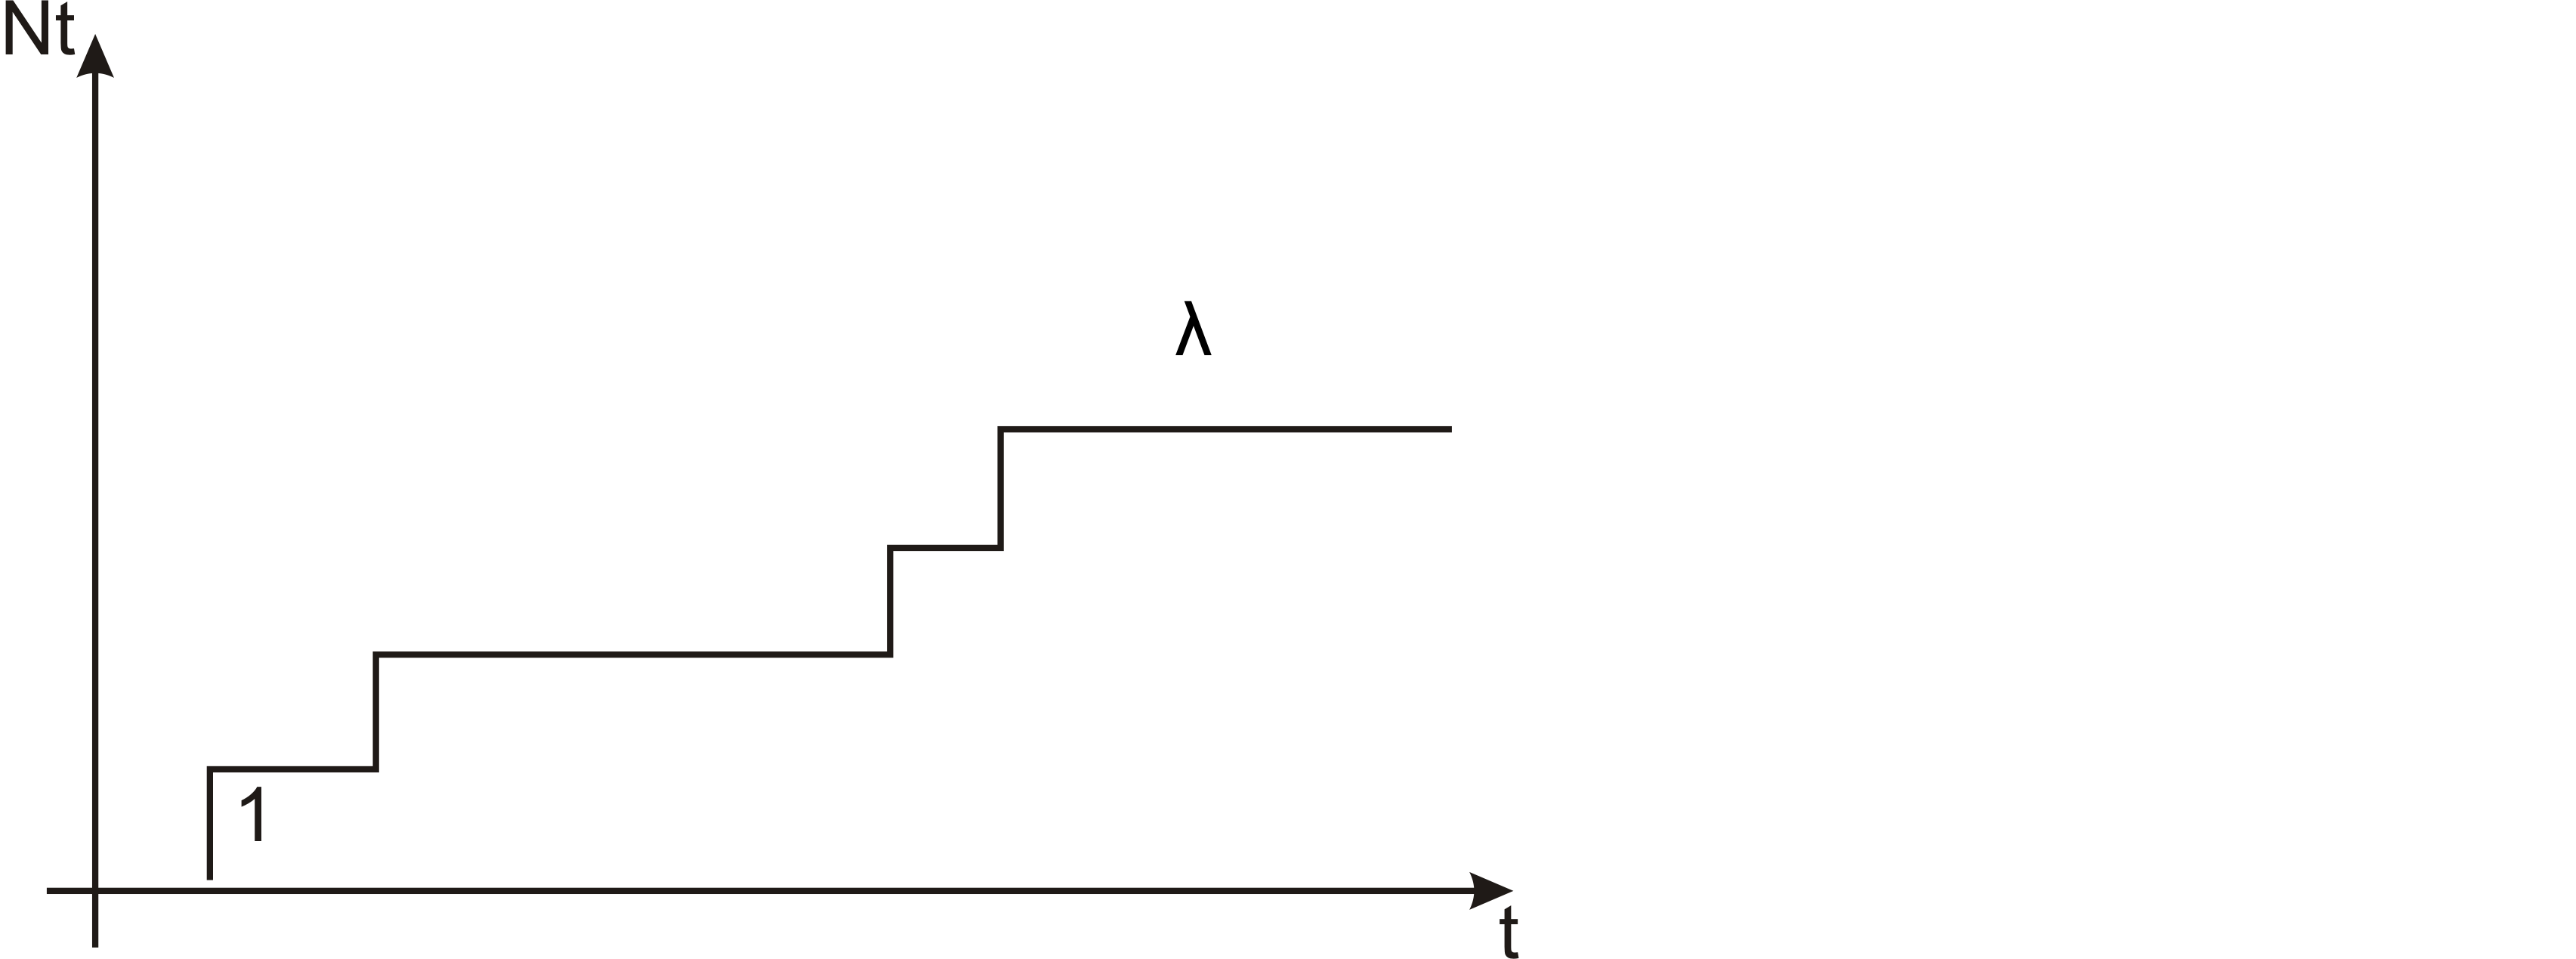
\includegraphics[width=4.5in]{Figures/rate.PNG}\\
 %% \caption{}\label{}
%\end{figure}
%Suppose $\{N_{t}, t \geq 0\}$ Poisson process with rate $\lambda$. 
%
%$\tilde{N_{t}}(w)= N_{t}(w)+f(t+X_{1}(w))$ where $f(t)$=0, if $t$ is irrational and $f(t)$=t, if $t$ is rational.\\
%\begin{eqnarray*}
%% \nonumber to remove numbering (before each equation)
  %P[\tilde{N_{t}}\neq N_{t}] &= P[\omega:t+X_{1}(\omega) \text{is rational}],\\
  %&= P[\omega:X_1(\omega)  \text{is rational} ] =0.
%\end{eqnarray*}
 
\end{document}